\documentclass{article}

\usepackage{url}

\usepackage{amssymb,amsfonts,amsmath,amsthm,mathtools}
\usepackage{adjustbox}
\usepackage{float}
\usepackage{caption}
\usepackage{mdframed}
\usepackage{lmodern}
\usepackage{bm,bbold}
\usepackage{xfrac, nicefrac}
\usepackage{xcolor}
\usepackage{lmodern}
\usepackage{enumitem}
\usepackage{pgfplots, pgf,tikz}
\usepackage[margin=60pt]{geometry}
\pdfinclusioncopyfonts=1
\captionsetup{width=0.85\textwidth}

\usepackage{pgfplots, pgf,tikz}
\usepgfplotslibrary{fillbetween}
\pdfinclusioncopyfonts=1
\captionsetup{width=0.85\textwidth}

\usepackage{xcolor}
\definecolor{RED}{HTML}{EB6231}
\definecolor{YELLOW}{HTML}{E29D26}
\definecolor{BLUE}{HTML}{5D80B4}
\definecolor{LIGHTGREEN}{HTML}{6ABD9B}
\definecolor{GREEN}{HTML}{8FB03E}
\definecolor{PURPLE}{HTML}{BE1E2D}
\definecolor{BROWN}{HTML}{A97C50}
\definecolor{PINK}{HTML}{DA1C5C}

\newcommand{\specialcell}[2][c]{%
	\begin{tabular}[#1]{@{}c@{}}#2\end{tabular}}

\DeclareMathOperator{\E}{\mathbb{E}}
\newcommand{\der}{\mathrm{d}}
\newcommand{\e}{\mathrm{e}}
\newcommand{\angstrom}{\text{\normalfont\AA}}

% Time, effective population size and mutation rate.
\newcommand{\Ne}{N_{\mathrm{e}}}
\newcommand{\dnds}{\omega}
\newcommand{\Nsite}{\text{n}}
\newcommand{\Nsites}{\text{n}}
\newcommand{\site}{\text{i}}
\newcommand{\Nstate}{\text{K}}

\newcommand{\x}{x}
\newcommand{\eq}{^{*}}
\newcommand{\dx}{\delta \x}
\newcommand{\s}{s}
\newcommand{\deltaG}{\Delta G}
\newcommand{\deltaGMin}{\alpha}
\newcommand{\deltadeltaG}{\Delta \deltaG}

\newcommand{\ci}{\mathbb{S}_{t}}
\newcommand{\cj}{\mathbb{S}_{t}'}
\newcommand{\itoj}{\ci, \cj}
\newcommand{\setNeighbors}{\mathcal{M}\left(\ci\right)}
\newcommand{\setNonSynNeighbors}{\mathcal{N}\left(\ci\right)}
\newcommand{\setSynNeighbors}{\mathcal{S}\left(\ci\right)}
\newcommand{\submatrix}{q}

\pgfplotsset{every axis/.append style={line width=1pt}}
\pgfplotscreateplotcyclelist{colors}{LIGHTGREEN\\YELLOW\\RED\\GREEN\\BLUE\\}

\begin{document}

\title{Substitution rate responses to changes in effective population size.}

\author{T. Latrille, N. Lartillot}
 
\maketitle
 
\abstract{
The quasi-neutral theory of evolution assert that the effective population size ($\Ne$) plays an important role in shaping the evolution of molecular sequences.
One consequence is that $\Ne$ modulates selection, such populations with high $\Ne$ would have stronger purifying selection, due to the decrease of random drift.
In molecular sequence, this effect translate in the decrease in the substitution rate of selected mutations relative to the substitution rate of neutral mutation ($\dnds$) with respect to $\Ne$.
Such theoretical prediction had been observed in empirical data across many clades.
However, several studies failed to observe such response of $\dnds$ to changes in $\Ne$, or with weak strength or direction.
Computational model of protein folding have shown that $\dnds$ can be independent of $\Ne$, which can mathematical be proven under certain assumptions.
Moreover, non-equilibrium properties can implies that an increase of $\Ne$ can result first in an increase of $\dnds$ and then a decrease.
Together, assumptions about the mapping of sequence to fitness can display a variety of behaviours in the $\dnds$ responses to changes in $\Ne$.
Our goal in this present work is to provide theoretical tools to derive the relationship between $\Ne$ and $\dnds$ in the context of a genotype-phenotype-fitness map.
We apply our framework in the case of fitness proportional to the probability of protein folding.
Our compact theoretical results match more complex simulations using 3d structure of proteins.
We assert that models based on the probability of folding are at odd with empirically results obtained on the $\Ne$-$\dnds$ relationship in population genetic dataset.
However, fitness function based on non-specific interactions between proteins match the empirical data.
We also stress the importance of epistatic interactions in the $\Ne$-$\dnds$ relationship, such that it determines to time to reach a new equilibrium, and that models without epistasis might be too slow to be realistic.
}

\section*{Introduction}
Differences in DNA sequences of a gene in separate species are due to the particular history of DNA substitutions along each specie's respective lineage.
These substitutions  at the level of the population are the result of point mutations at the level of individuals, subject to evolutionary forces such as selection and random drift.
In protein-coding DNA sequences, non-synonymous mutations are changing the amino-acid sequence, and by comparing the non-synonymous substitutions rate relative to the synonymous substitution rate (supposedly neutral), a statistic called $\dnds$, we can estimate the global strength of selection and random drift.\\

For a given gene, it has been empirically observed changes of $\dnds$ along lineages of a phylogeny \cite{Yang2001, Zhang2004}.
More importantly, changes in substitution rate correlate with changes in life-history-traits (longevity, body mass, ...) such as shown by the molecular comparative framework \cite{Lartillot2011,Weber2014}.
Such covariation are compatible with the theoretical prediction of the nearly-neutral theory of evolution \cite{Ohta1972, Ohta1992}, where the underlying mechanism is changes in effective population size ($\Ne$).
Indeed, populations with low $\Ne$ would have both a large body size and a high $\dnds$ (weaker selection) due to the increase of random drift.
If $\dnds$ is empirically correlated to life-history traits, such as body mass and longevity, the direction of correlation could not be replicated across all experiments \cite{Figuet2016}.\\

Theoretical prediction of $\dnds$ decreasing as a function of $\Ne$ had been developed in the context of a fixed distribution of fitness effects \cite{Ohta1972, Welch2008}, and also been shown in context of a fixed fitness landscape, where each amino-acid have different fitnesses \cite{Spielman2015a, DosReis2015}.
However, it has also been argued that the existence of a $\dnds$ response to $\Ne$ is not straightforward, even in the context of nearly-neutral theory of evolution \cite{Lanfear2014}.
In the example of a bio-chemical mechanistic computational model, where the fitness is determined by the probability of folding, $\dnds$ is independent of $\Ne$ \cite{Goldstein2013}.
Theoretically, a more general case is obtained whenever the fitness is a concave function of a trait, and such trait is equimutable \cite{Cherry1998}.
Equimutabibilty meaning a mutation has the same effect on the trait whatever the current trait of the individual.
Moreover, even in the case of a $\dnds$ response to $\Ne$, this response is far from being $1$-to-$1$ due to non-equilibrium properties, such that an increase in $\Ne$ implies firstly a burst of $\dnds$, and subsequentially a decrease in $\dnds$ \cite{Jones2016}.\\

Our goal in this present work to reconcile empirical observation with theoretical results, such as to delimit which models and assumptions are reasonable.
This question is important if we want to extract changes in effective population size from substitution history, as well as to determine the fitness landscape under which protein-coding DNA sequences are evolving.
We provide theoretical tools to derive the relationship between $\Ne$ and $\dnds$ in the context of a genotype-phenotype-fitness map.
We apply our framework in the case of fitness proportional to the probability of protein folding.
Our compact theoretical results match more complex simulations using 3d structure of proteins.
We assert that models based on the probability of folding are at odd with empirically results obtained on the $\Ne$-$\dnds$ relationship in population genetic dataset.
However, fitness function based on non-specific interactions between proteins match the empirical data.
We also stress the importance of epistatic interactions in the $\Ne$-$\dnds$ relationship, such that it determines to time to reach a new equilibrium, and that models without epistasis might be too slow to be realistic.

\section*{Results}
\subsection*{Theoretical approximations}

We seek to determine the change in $\dnds$ at equilibrium after a change in $\Ne$.
This model map the amino-acid sequence to a phenotype $\x$, in this case the proportion of unstable sites in the protein. Each site can be in one of $\Nstate \geq 2$ states, where only $1$ state is defined the stable state, and $\Nstate - 1$ states are unstable. After a mutation, given that only one site can change at a time, the absolute change of $\x$ is either $0$ or $\dx=\sfrac{1}{\Nsite}$, where $\Nsite$ is the number of sites. The Wrightian fitness of phenotype $\x$ is called $f(\x)$
We demonstrate (See Supplementary Materials) that: 
\begin{align}
\frac{ \der \omega\eq}{\der \ln (\Ne)} & \simeq - \frac{\frac{ \partial \ln f(\x\eq) }{\partial {\x\eq}}}{\frac{ \partial^2 \ln f(\x\eq) }{\partial {\x\eq}^2}},
\end{align}
where $\x\eq$ is the phenotype value at equilibrium.
Thus, the slope of the $\dnds$ elasticity to changes in $\Ne$ is the ratio of first to second derivative of the log-fitness function. Moreover, the equilibrium value of $\x\eq$ is given by the equation:
\begin{align}
\ln \left( \frac{1 - \x\eq}{\x\eq} \right) + \ln (\Nstate-1) \simeq - \frac{4\Ne}{\Nsite} \frac{ \partial \ln f(\x\eq) }{\partial {\x\eq}}
\end{align}
As an example, Wrightian fitness is defined as the probability of our protein to be in the folded state, given by fermi dirac distribution: 
\begin{equation}
f(\x) = \dfrac{1}{1 + e^{\beta (\deltaGMin + \Nsite * \gamma * \x)}}, 
\end{equation} .
where $\deltaGMin$ and $\gamma$ are in kcal/mol, and the fixed parameter $\beta=1.686$ mol/kcal at room temperature. Thus, $\deltaGMin < 0$ is the difference in free energy between folded and unfolded state when all sites are stable. $\Nsite \gamma > 0$ is the expected change in free energy (between folded and unfolded states) when all sites are unstable.

\begin{figure*}[htb!]
	\begin{mdframed}
		\centering
		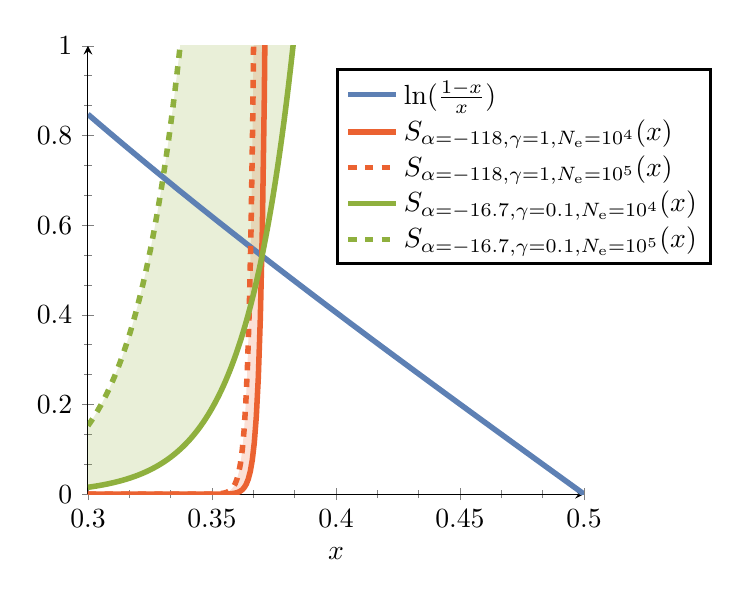
\begin{tikzpicture}
		\begin{axis}[
		width=0.65\textwidth,
		height=\axisdefaultheight,
		xlabel={$\x$},
		ymin=0.0, ymax=1.0,
		samples=100,
		legend entries={$\ln(\frac{1 - \x}{\x})$,
			$S_{\deltaGMin = -118, \gamma = 1,\Ne = 10^{4}}(\x)$,
			$S_{\deltaGMin = -118, \gamma = 1,\Ne = 10^{5}}(\x)$,
			$S_{\deltaGMin = -16.7, \gamma = 0.1,\Ne = 10^{4}}(\x)$,
			$S_{\deltaGMin = -16.7, \gamma = 0.1,\Ne = 10^{5}}(\x)$,
		},
		legend cell align=left,
		minor tick num=2,
		axis x line=bottom,
		axis y line=left,
		legend style={at={(0.5,0.95)},anchor=north west}
		]
		\addplot[domain=0.3:0.6,line width=2.0pt, color=BLUE]{ ln((1-x)/x) };
		\addplot[name path=A, domain=0.3:0.38, line width=2.0pt, color=RED]{4*10000*1.686*exp(1.686*(-118+300*x))};
		\addplot[name path=B, dashed,domain=0.3:0.37, line width=2.0pt, color=RED]{4*100000*1.686*exp(1.686*(-118+300*x))};
		\addplot[name path=C,domain=0.3:0.39, line width=2.0pt, color=GREEN]{4*10000*0.1*1.686*exp(1.686*(-16.71+30*x))};
		\addplot[name path=D,dashed,domain=0.3:0.35, line width=2.0pt, color=GREEN]{4*100000*0.1*1.686*exp(1.686*(-16.71+30*x))};
		\addplot[fill=RED, opacity=0.2] fill between[ of = A and B];
		\addplot[fill=GREEN, opacity=0.2] fill between[ of = C and D];
		\end{axis}
		\end{tikzpicture}
		\caption{
			\textbf{$\bm{\dnds}$ response to change in $\bm{\Ne}$}.
			The equilibrium $\x\eq$ is determined by the equation $\ln(\frac{1 - \x\eq}{\x\eq})=S_{\deltaGMin,\Nsite \gamma,\Ne}(\x\eq)$ (see Supplementary Materials). $S$ is proportional to $\Ne$, but increase exponentially with $\x$ where $\Nsite \gamma$ is the exponential growth rate.
		}
		\label{fig:NeChangeInfluence}
	\end{mdframed}
\end{figure*}
With such fitness function, we have (See Supplementary Materials) :
\begin{equation}
\frac{ \der \omega\eq}{\der \ln (\Ne)} \simeq -\dfrac{1}{\beta \Nsite \gamma}.
\end{equation}
which is independent of $\x\eq$, meaning $\omega$ is linearly decreasing with $\Ne$ in log space.
Meaning that under a value of $\Nsite=300$ sites, $\gamma=1.0$ kcal/mol, the slope of the linear relationship between $\dnds$ and log-$\Ne$ is $0.002$.

\subsection*{Simulations confirmation}
We compare our model to the original studies \cite{Williams2006, Goldstein2011, Pollock2012}, where free energy of the folded state is computed using the $3$D structure of the folded state and pair-wise contact potential energies between neighboring amino-acid residues \cite{Miyazawa1985}.
The free energy distribution of unfolded states is approximated using $55$ decoy $3$D structures that supposedly represent a sample of possible unfolded states (see Supplementary Materials).

\begin{figure*}[htb!]
\begin{mdframed}
\centering
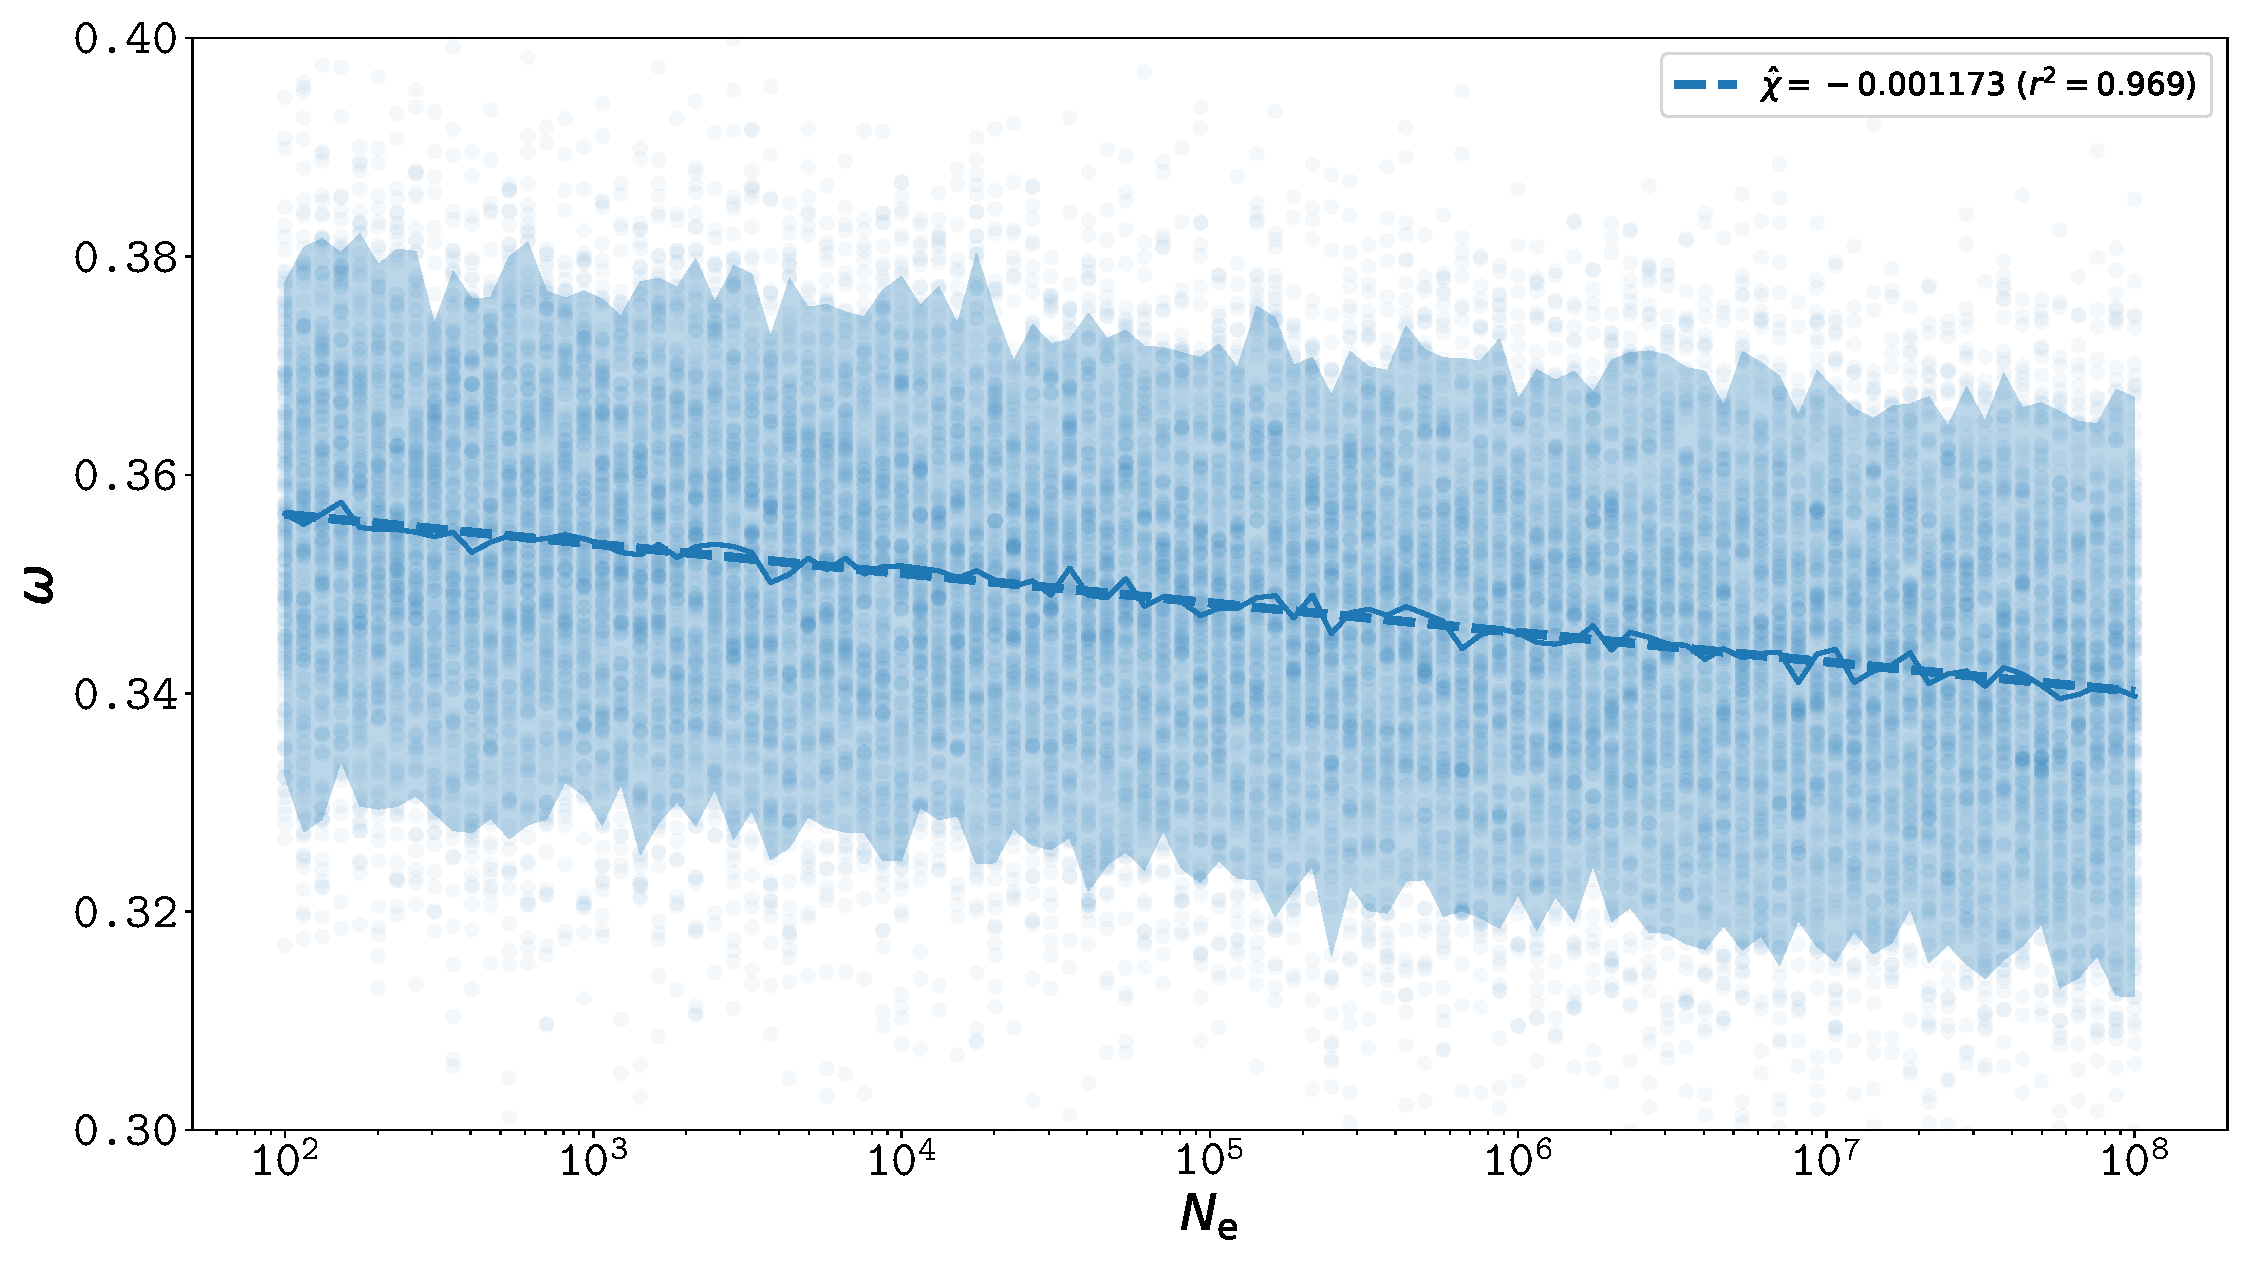
\includegraphics[width=0.8\textwidth] {artworks/SimuFold-Elasticity.pdf}
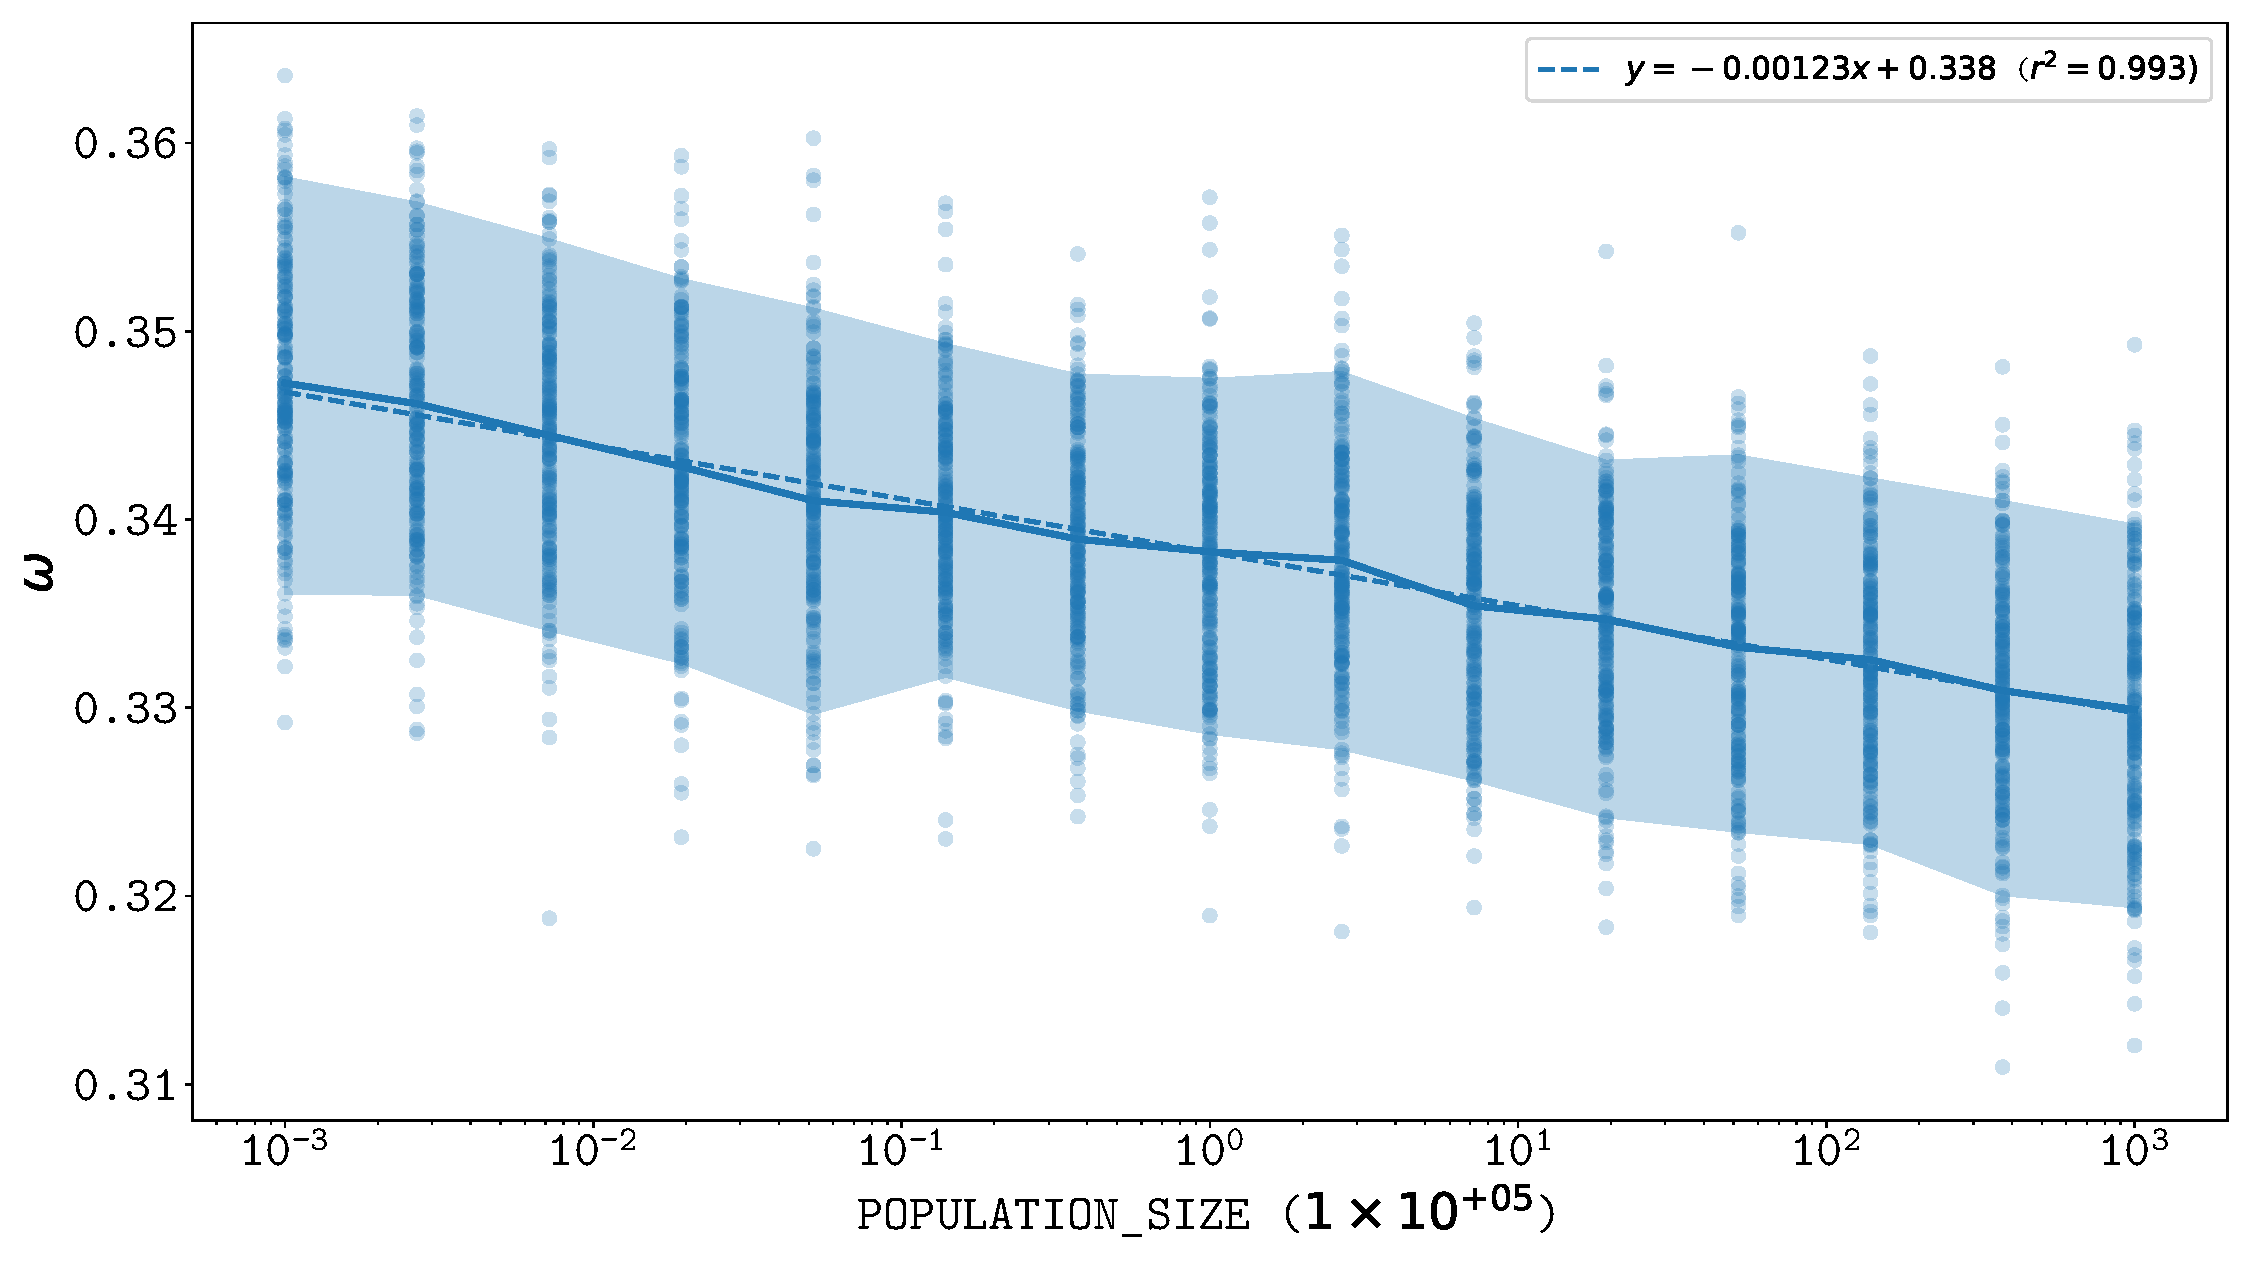
\includegraphics[width=0.8\textwidth] {artworks/SimuStab-Grantham-Elasticity.pdf}
	\caption{
		\textbf{$\bm{\dnds}$ elasticity to change in $\bm{\Ne}$}.
		For each population size, $200$ simulations were performed and the average (solid line) and $90\%$ confidence interval (shaded area) are shown.
		In the model of 3D free energy of folding, $\dnds$ at equilibrium is weakly dependent on log-$\Ne$ but is not independent as claimed originally \cite{Goldstein2013}.
		This weak dependence matches the theoretical prediction of our additive free energy model that the linear relation (dashed line) has a slope equal to $(\beta  \Nsite \gamma)^{-1} = 0.00198 \simeq 0.00124$.
		Bottom panel, The fixed parameters are $\alpha=-118$, $\gamma=1$, $\Nsite=300$, $\beta=1.686$, and for each non-optimal amino-acid, $\gamma$ is scaled by the Grantham distance to the optimal amino-acid.
		Moreover, with the Grantham model, the $\dnds$ matches the empirical 3D model of Golstein \& Pollock and the theoretical prediction.
		\label{fig:GoldsteinVsToy}
	}
\end{mdframed}
\end{figure*}
Simulations of protein evolution with both models display the same $\dnds$-$\Ne$ relationship, whenever the parameters $\alpha$ and $\gamma$ of our model are set to match the average values of the $3$D model (see Figure \ref{fig:EqdndsNe}).
In such experiment, $\alpha=-118$ kcal/mol as it is the $\deltaG$ of the most stable sequence of $300$ sites \cite{Goldstein2011}.
The parameter is set $\gamma=1.0$ kcal/mol, the average observed increase in $\deltaG$ per destabilizing mutation \cite{Zeldovich2007}.
The original works claimed that under the $3$D model, $\dnds$ is independent of $\Ne$ because $\deltaG$ is an equimutable parameter.
We argue instead that $\dnds$ is approximatively linear with log-$\Ne$, and that $\deltaG$ is not equimutable (see Figure \ref{fig:EqdndsNe}).
Thus if we consider $\deltadeltaG = 1.0$ kcal/mol for destabilizing mutations, the slope is determined solely by the number of sites in the protein. 


\subsection*{Epistasis determines the time to relaxation}

Although the equilibrium value of $\dnds$ after changes in $\Ne$ is an important feature of the $\dnds$-$\Ne$ relationship, an other parameter that is often neglected is the relaxation time to reach the new equilibrium $\dnds$ \cite{Jones2016}.
\begin{figure*}[htb!]
\begin{mdframed}
	\centering
	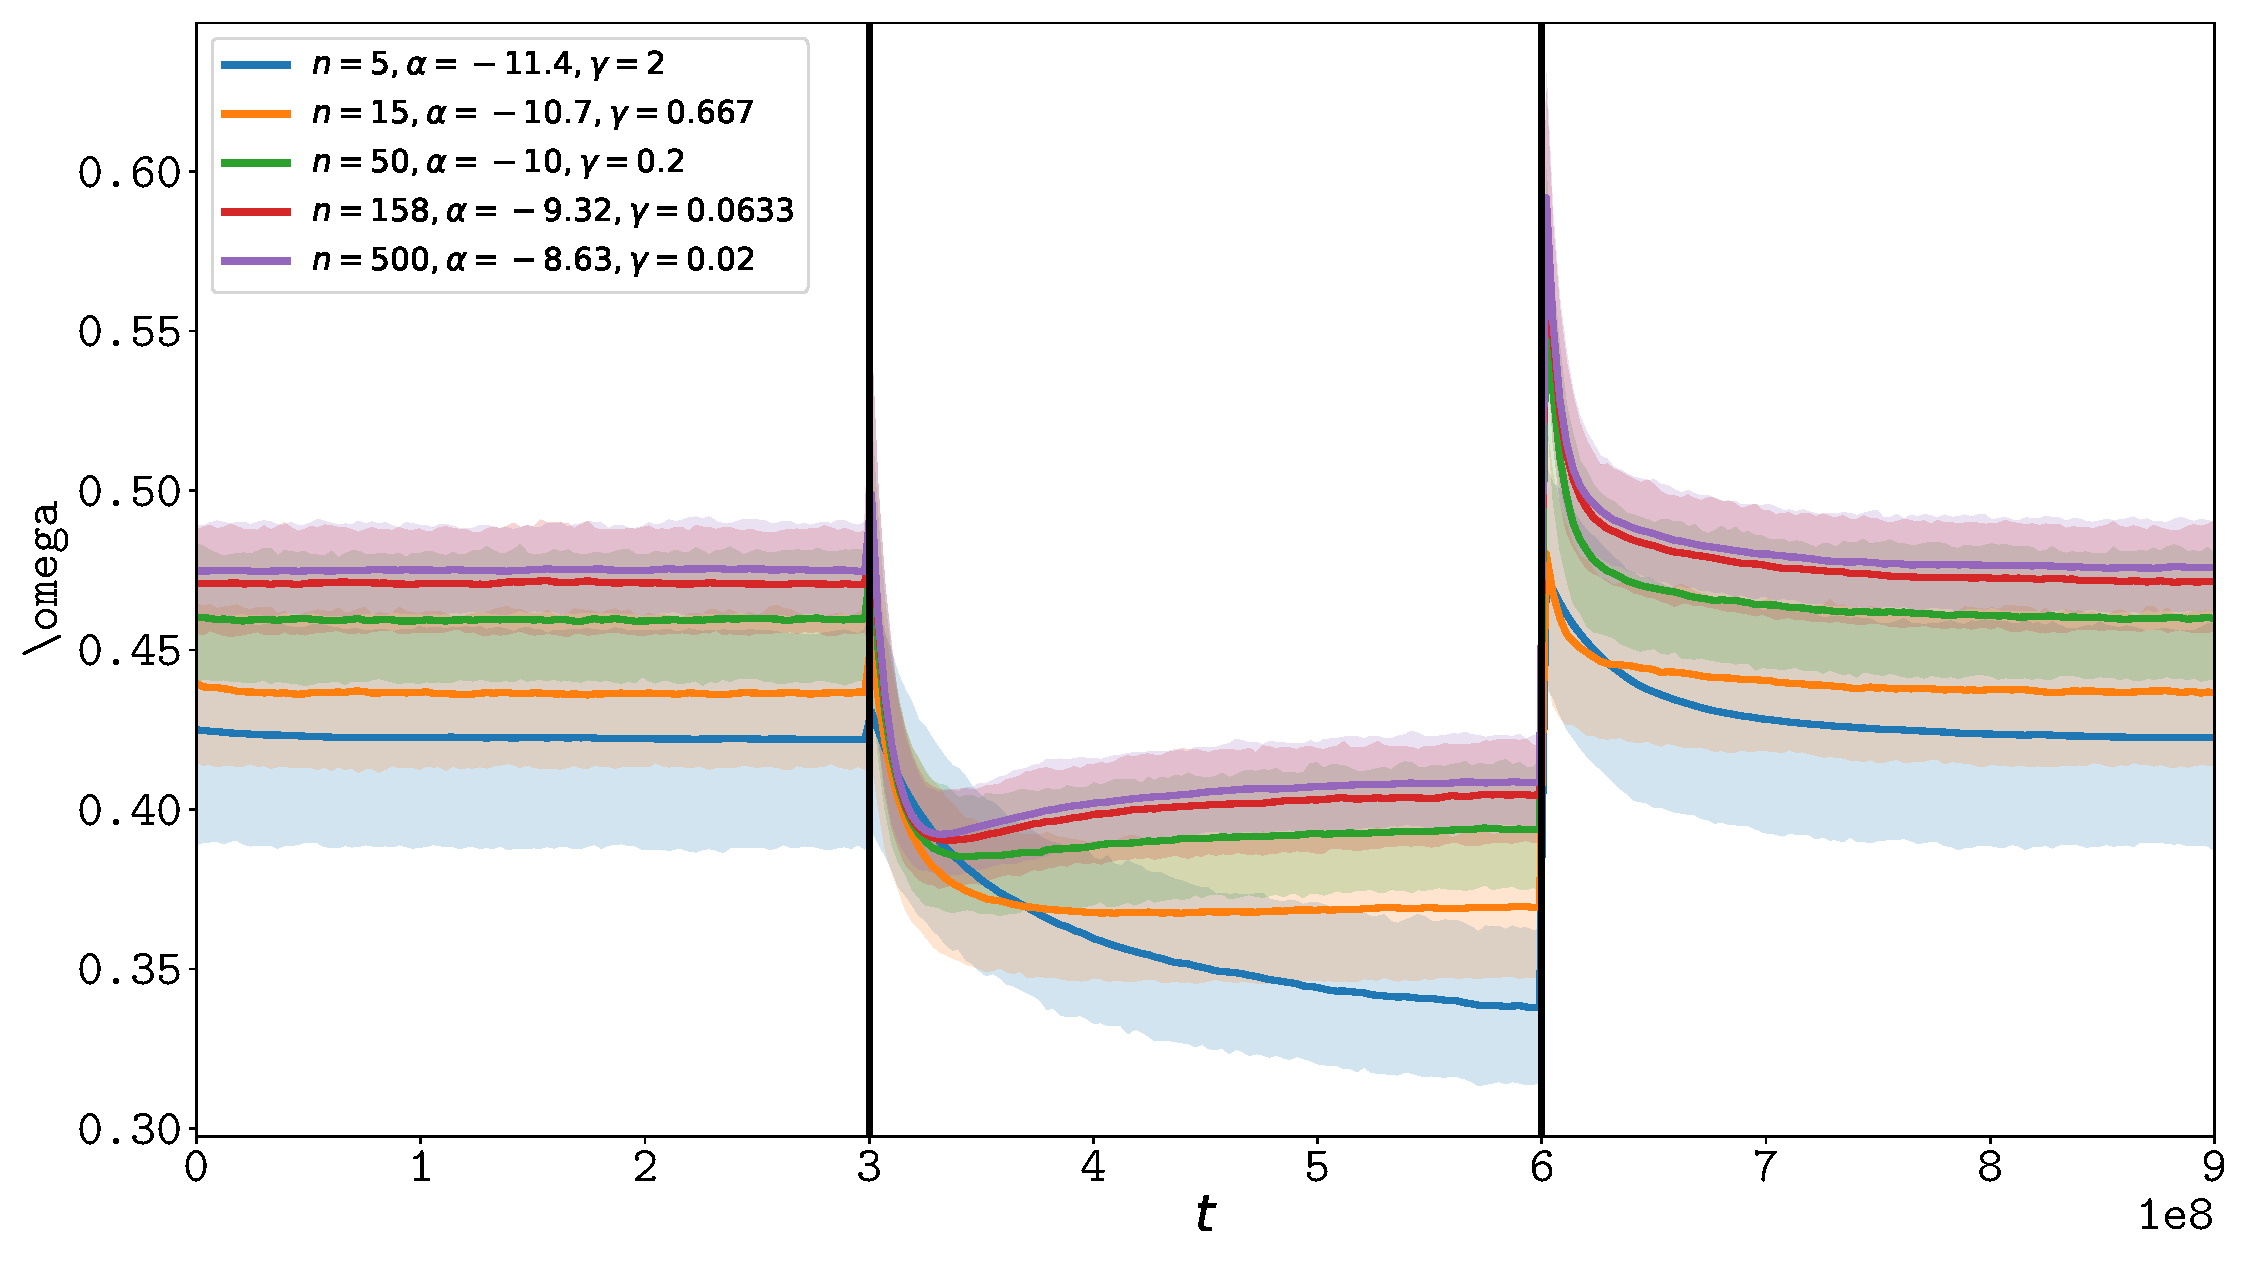
\includegraphics[width=0.8\textwidth] {artworks/Relaxation-Stability-Alpha-Gamma.pdf}
	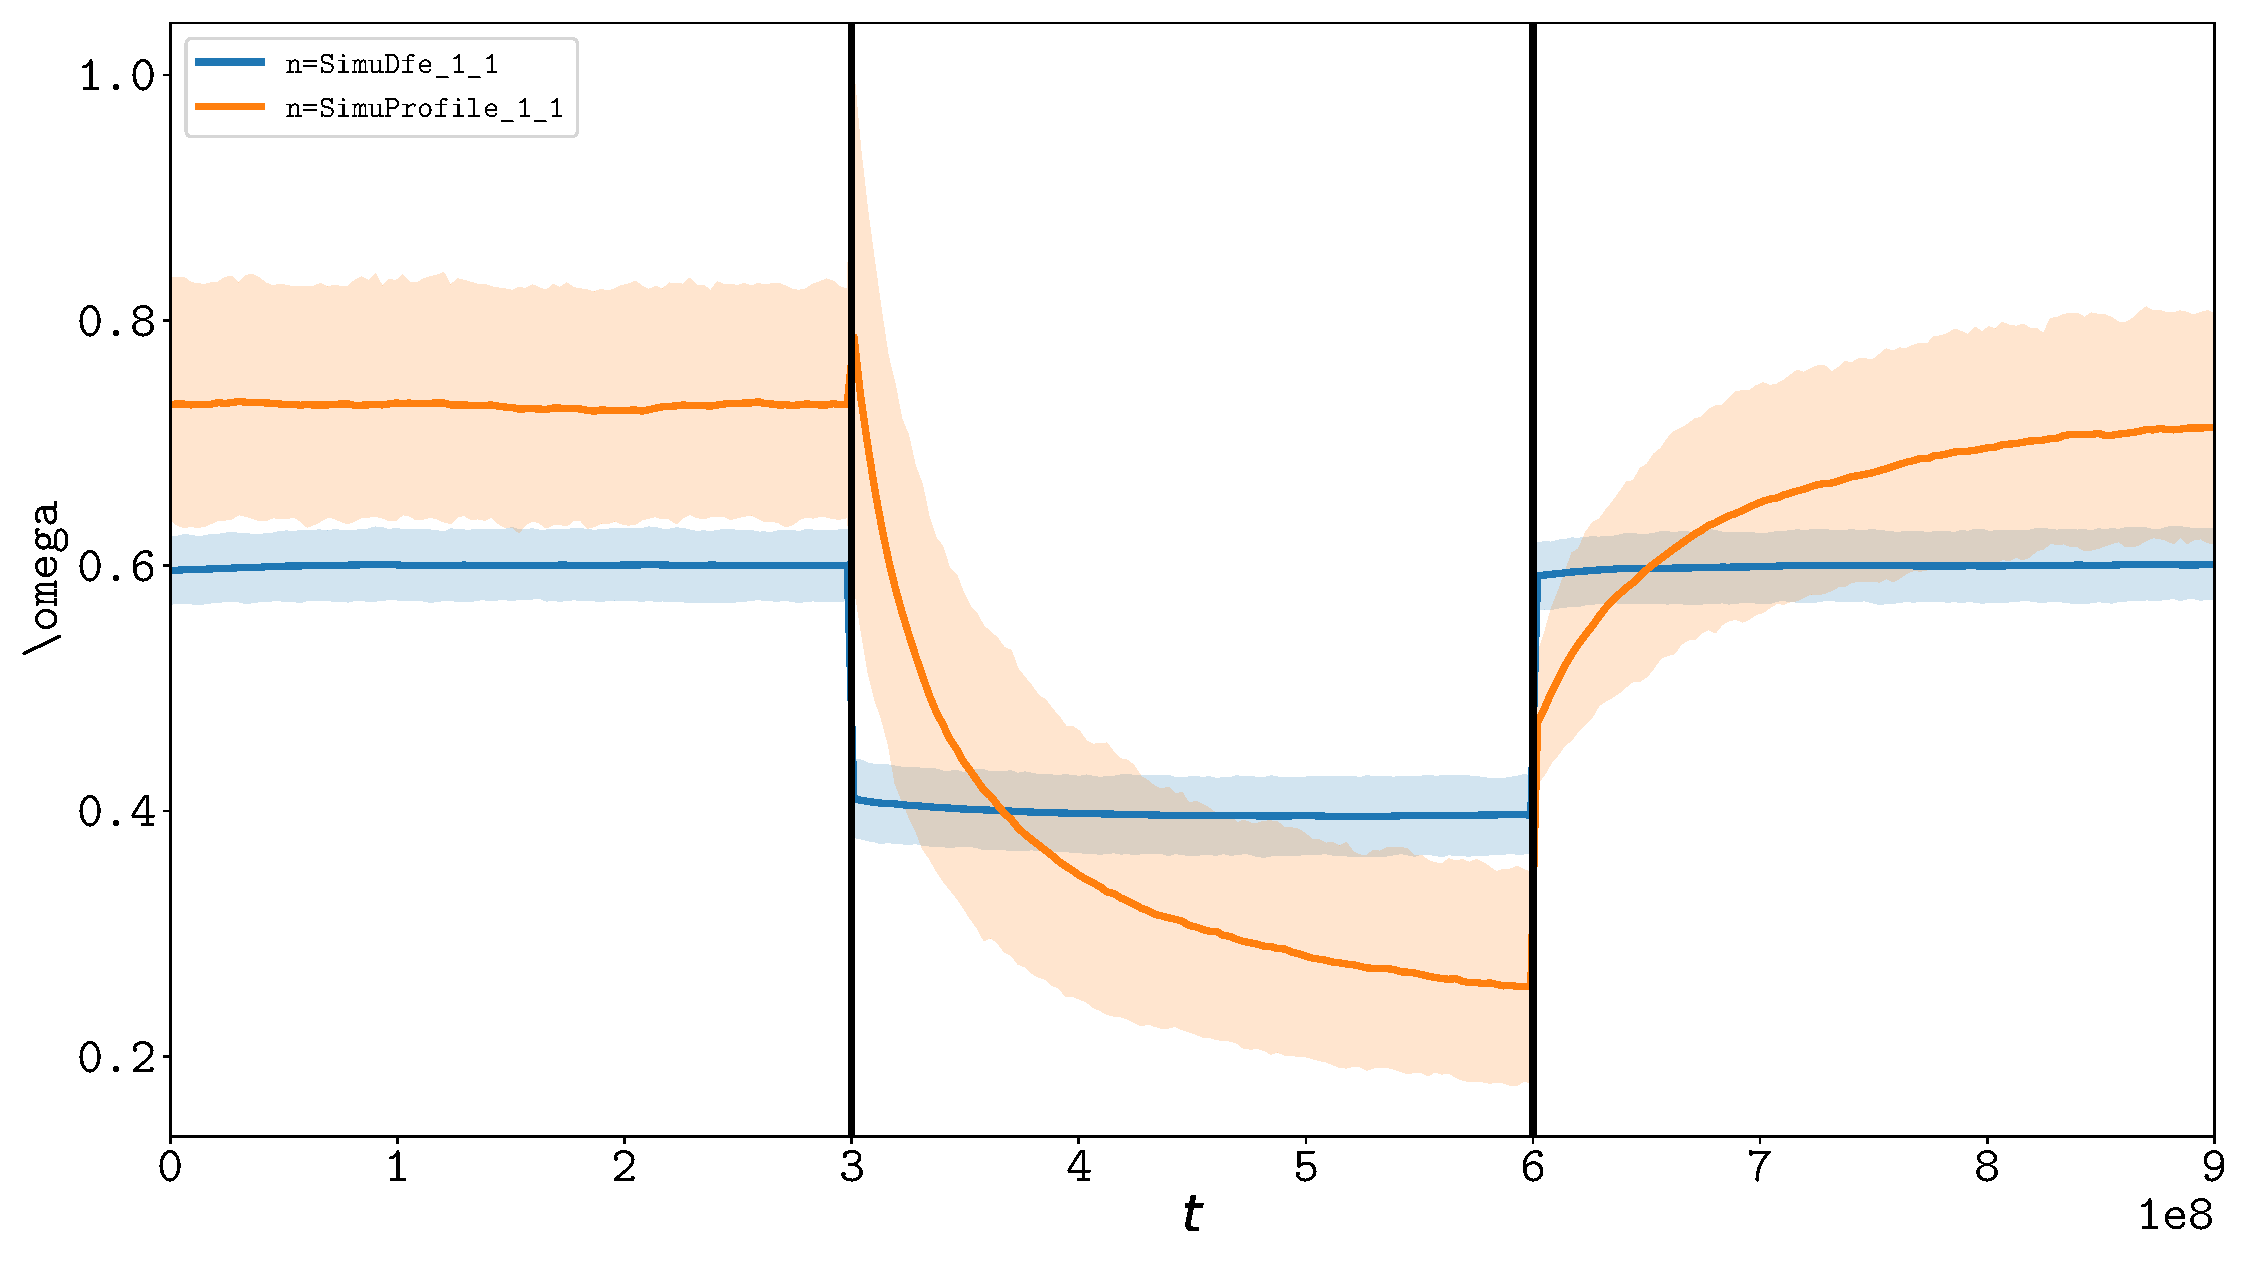
\includegraphics[width=0.8\textwidth] {artworks/Relaxation-DFE-Profile-N50.pdf}
	\caption{
		\textbf{$\bm{\dnds}$ relaxation time to changes in $\bm{\Ne}$}.
		Top panel. $\dnds$ relaxation after a brutal change in $\Ne$, the left and right panel correspond to low $\Ne$ ($1e^{5}$) and the middle panel corresponds to high $\Ne$ ($2e^{6}$). 
		Solid line correspond to the average over replicates ($r$) and the shaded area correspond to the $90\%$ interval among replicates. 
		The mutation rate ($\mu$) is $1e{-8}$ per year per site, and the total time of the computation is $900$ million years.
		$\beta=1.686$, $\gamma=-10$ for all simulations. The number of sites is changed from $\Nsite=15$ to $\Nsite=158$, and the number of replicates is changed accordingly such that the total number of sites ($\Nsite*r$) is kept constant.
		Moreover, $\gamma$ is changed according to $\Nsite$ such that the product $\gamma\Nsite$ is kept constant, thus the  elasticity of the $\dnds$ to changes in $\Ne$ is kept constant.
		Finally, $\alpha$ is changed according to $\Nsite$ and $\gamma$ such that the equilibrium value $\x\eq$ is kept constant, by solving numerically equation \ref{eq:equilibrium}.
		Increasing $\Nsite$ implies a higher rate of relaxation.
		Panel B.  In context of a fixed fitness landscape, where each amino-acid have different fitnesses (site-specific profile), the time taken to reach the new equilibrium value of $\dnds$ after a change in $\Ne$ is long, such that relaxation rate is on the order of the mutation rate. In the context of a distribution of fitness effects, the relaxation time is non-existent.
	}
	\label{fig:relaxStability}
\end{mdframed}
\end{figure*}
In the case of a fitness landscape with epistasis, after a change in $\Ne$, any site that is used to climb either up or down the fitness landscape will have diminishing return in other site of the sequences.
Not taking into account epistasis have the consequence of over-estimating the relaxation time to return to equilibrium of $\dnds$ after changes in $\Ne$ \ref{fig:relaxStability}).

Using a site-specific fitness landscape, where each amino-acid have different fitnesses, thus with no epistasis, the relaxation time is long since every site has to adapt to the new change in $\Ne$.
However, using a distribution of fitness effect (DFE) does not suffer from under-estimating the relaxation rate, since the effect is instantaneous (see Figure \ref{fig:relaxProfileDFE}).

\section*{Discussion}

Goldstein \& Pollock argued that model of protein evolution should consider how the acceptance of mutations depends on the sequence context in which they arise (epistasis), as to correctly represent resultant rate heterogeneity along the sequence, to predict the role of compensatory substitutions in protein evolution, predict which of the 10\% of deleterious mutations in humans are harmless in other species, or to accurately represent the rate and time dependence of convergence and homoplasy \cite{Goldstein2017}.
We argue that not taking into account epistasis also have the consequence of over-estimating the relaxation time to return to equilibrium of $\dnds$ after changes in $\Ne$.
Paradoxically, not taking into account epistasis means over-estimating the response of $\dnds$ to changes in $\Ne$ at equilibrium.\\

If using a distribution of fitness effect (DFE) is mathematically convenient and does not suffer from under-estimating the relaxation rate, it is also over-estimating the response of $\dnds$ to changes in $\Ne$ at equilibrium (\textit{should show proof and mechanistic explanation that the selection coefficient shall not be independent of $\Ne$}).
As such, developing inference of fitness landscape will require to assume site-interdependent fitness landscapes.\\

Our model does not display site variation in $\dnds$, which is a strong limitation, as it has observed in most protein \cite{Echave2017}.
\section*{Materials \& Methods}

Protein sequence evolution are simulated under an origin-fixation model \cite{McCandlish2014}., where the rate of substitution of a new mutation with selection coefficient $s$ is:
\begin{equation}
p_{\text{fix}}(s) = \mu \dfrac{4 \Ne s}{1 + e^{- 4 \Ne s }}, 
\end{equation}
where $\mu$ is the mutation rate.

\subsection*{Simulation of protein folding with an additive model of free energy}
\label{MatMet:folding}
From a DNA sequence $\ci$ after $t$ substitutions, the protein's difference in free energy between folded and unfolded state is given by:
\begin{equation*}
\deltaG\left(\ci\right) = \deltaGMin + \Nsite \gamma * \x\left(\ci\right), 
\end{equation*}
where $\x\left(\ci\right)$ is the proportion of non-optimal amino-acid sites in the sequence.
Wrightian fitness is defined as the probability of our protein to be in the folded state, given by the Boltzmann equation: 
\begin{equation}
f(\deltaG\left(\ci\right)) = \dfrac{P_{\mathrm{F}}\left(\ci\right)}{P_{\mathrm{F}}\left(\ci\right) + P_{\mathrm{U}}\left(\ci\right)} = \dfrac{e^{-\beta G_{\mathrm{F}}\left(\ci\right) }}{e^{-\beta G_{\mathrm{F}} \left(\ci\right) } + e^{-\beta G_{\mathrm{U}}\left(\ci\right) }} = \dfrac{1}{1 + e^{\beta \deltaG\left(\ci\right) }}, 
\end{equation}
where $\beta$ is the inverse of the temperature ($\beta=1/kT$).

From the resident sequence $\ci$, we define $\setNeighbors$ as the set of all possible mutant that are one nucleotide away from $\ci$, and were mutant sequences containing a stop codon are excluded.
For a protein of $\Nsite$ amino-acid sites, $\left| \setNeighbors \right| \leq 9 \Nsite$, since each codon has a maximum of $9$ possible mutant codon that are one mutation away and that are not stop codon.
For each mutant sequence $\cj \in \setNeighbors$, we compute $\deltaG^{t+1}$ from the updated sequence $\cj$, and subsequently the selection coefficient of the mutant:
\begin{equation}
s \left( \ci,\cj\right) = \dfrac{ f\left( \deltaG \left(\cj\right) \right) - f\left( \deltaG \left(\ci\right) \right)}{f\left( \deltaG \left(\ci\right) \right)}.
\end{equation}
The next change in the protein coding DNA and the time to next the event is chosen using Gillespie algorithm, according to the rates of substitution between codons:
\begin{equation}
\submatrix_{\itoj} = \mu_{\itoj} \dfrac{4 \Ne s \left( \ci,\cj\right)}{1 - \e^{-4 \Ne s \left( \ci,\cj\right)}}, 
\end{equation}
where $\mu_{\itoj}$ is the mutation rate between $\ci$ and $\cj$, determined by the underlying $4x4$ nucleotide mutation rate matrix, and ${\submatrix_{\itoj}} = \mu_{\itoj}$ in the case of synonymous substitutions.

\subsection*{Simulation with independent fitness profiles}
A fitness profile give a fitness for each amino-acid (vector of size $20$).
Each site of the protein has a specific amino-acid fitness profile.
Overall, the protein phenotype is computed as the sum of site-specific selection coefficient, obtained by accessing the amino-acid present at each site of the protein.
The selection coefficient of the mutant $\cj$ is:
\begin{equation}
s \left( \ci,\cj\right) = \sum_{1 \leq \site \leq \Nsite} \ln \left( \dfrac{G_{\site} \left(\cj(\site) \right)}{G_{\site} \left(\ci(\site) \right)} \right) ,
\end{equation}
where $G_{\site}$ is the fitness profile at site $\site$, obtained in empirical experiment \cite{Bloom2017}.
The next change in the protein coding DNA and the time to next the event is chosen using Gillespie algorithm, as in \ref{MatMet:folding}.

\subsection*{Simulation with distribution of fitness effects (DFE)}
The selection coefficient of the mutant $\cj$ is gamma distributed (shape $\beta > 0$):
\begin{equation}
- s \left( \ci,\cj\right) \sim \text{Gamma} \left( \bar{|s|}, \beta \right)
\end{equation}
The next change in the protein coding DNA and the time to next the event is chosen using Gillespie algorithm, as in \ref{MatMet:folding}.

\subsection*{$\bm{\dnds}$ along the simulation}
From the set of mutant $\setNeighbors$ that are one nucleotide away from $\ci$, we define the subsets $\setNonSynNeighbors$ and $\setSynNeighbors$ that are respectively the set of non-synonymous and synonymoys mutants, where  $\setNonSynNeighbors \cup \setSynNeighbors = \setNeighbors$.
As in previous works \cite{Spielman2015a, DosReis2015, Jones2016}, the ratio of non-synonymous over synonymous substitution rates of the sequence is defined as :
\begin{align}
\dnds(t) &= \dfrac{\sum_{\cj \in \setNonSynNeighbors} \submatrix_{\itoj}}{\sum_{\cj \in \setNonSynNeighbors} \mu_{\itoj}} \left( \dfrac{\sum_{\cj \in \setSynNeighbors} \submatrix_{\itoj}}{\sum_{\cj \in \setSynNeighbors} \mu_{\itoj}} \right)^{-1}\\
 &= \dfrac{\sum_{\cj \in \setNonSynNeighbors} \mu_{\itoj} \dfrac{4 \Ne s \left( \ci,\cj\right)}{{1 - \e^{-4 \Ne \left( \ci,\cj\right)} }}}{\sum_{\cj \in \setNonSynNeighbors} \mu_{\itoj}} 
\end{align}
\subsection*{Reproducibility}
The simulators written in C++ are publicly available under MIT license at \url{https://github.com/ThibaultLatrille/SimuEvol}.
The scripts and instructions necessary to reproduce the experiments are available at \url{https://github.com/ThibaultLatrille/GenotypePhenotypeFitness}.

\bibliographystyle{apalike}
\bibliography{refs-codons,refs-cds}



\end{document}